\section{\IFRU{Уровень}{Level} 2}

\IFRU{Для решения задач второго уровня, вам вероятно понадобится текстовый редактор или тетрадка с ручкой}
{For solving exercises of level 2, you probably will need text editor or paper with pencil}.

\subsection{\Exercise 2.1}
% toupper()

\index{OpenWatcom}
\IFRU{Это стандартная функция из библиотек Си. Исходник взят из OpenWatcom}.
{This is standard C library function. Source code taken from OpenWatcom}.

\subsubsection{MSVC 2010}

\lstinputlisting{exercises/1_1_msvc.asm}

\subsubsection{GCC 4.4.1 + \Othree}

\lstinputlisting{exercises/1_1_gcc.asm}

\subsubsection{Keil (ARM) + \Othree}

\lstinputlisting{exercises/1_1_ARM.s}

\subsubsection{Keil (thumb) + \Othree}

\lstinputlisting{exercises/1_1_thumb.s}

\subsection{\Exercise 2.2}
% atoi()

\index{OpenWatcom}
\IFRU{Это также стандартная функция из библиотек Си. Исходник взят из OpenWatcom и немного переделан}. 
{This is also standard C library function. Source code is taken from OpenWatcom and modified slightly}.

\IFRU{Эта функция использует стандартные функции Си:}
{This function also use these standard C functions:} isspace() \AndENRU isdigit().

\subsubsection{MSVC 2010 + \Ox}

\lstinputlisting{exercises/1_2_msvc.asm}

\subsubsection{GCC 4.4.1}

\IFRU{Задача немного усложняется тем, что GCC представил isspace() и isdigit() 
как inline-функции и вставил их тела прямо в код.}
{This exercise is slightly harder since GCC compiled isspace() and isdigit()
functions as inline-functions and inserted their bodies right into the code.}

\lstinputlisting{exercises/1_2_gcc.asm}

\subsubsection{Keil (ARM) + \Othree}

\lstinputlisting{exercises/1_2_ARM.s}

\subsubsection{Keil (thumb) + \Othree}

\lstinputlisting{exercises/1_2_thumb.s}

\subsection{\Exercise 2.3}
% rand()/srand()

\IFRU{Это также стандартная функция из библиотек Си, а вернее, две функции, работающие в паре. 
Исходник взят из MSVC 2010 и немного переделан.}
{This is standard C function too, actually, two functions working in pair.
Source code taken from MSVC 2010 and modified slightly.}

\IFRU{Суть переделки в том, что эта функция может корректно работать в мульти-тредовой среде, 
а я, для упрощения (или запутывания) убрал поддержку этого.}
{The matter of modification is that this function can work properly in multi-threaded environment,
and I removed its support for simplification (or for confusion).}

\subsubsection{MSVC 2010 + \Ox}

\lstinputlisting{exercises/1_3_msvc.asm}

\subsubsection{GCC 4.4.1}

\lstinputlisting{exercises/1_3_gcc.asm}

\subsubsection{Keil (ARM) + \Othree}

\lstinputlisting{exercises/1_3_ARM.s}

\subsubsection{Keil (thumb) + \Othree}

\lstinputlisting{exercises/1_3_thumb.s}

\subsection{\Exercise 2.4}
% strstr()

\IFRU{Это стандартная функция из библиотек Си. Исходник взят из MSVC 2010.}
{This is standard C library function. Source code taken from MSVC 2010.}

\subsubsection{MSVC 2010 + \Ox}

\lstinputlisting{exercises/1_4_msvc.asm}

\subsubsection{GCC 4.4.1}

\lstinputlisting{exercises/1_4_gcc.asm}

\subsubsection{Keil (ARM) + \Othree}

\lstinputlisting{exercises/1_4_ARM.s}

\subsubsection{Keil (thumb) + \Othree}

\lstinputlisting{exercises/1_4_thumb.s}

\subsection{\Exercise 2.5}
% Pentium FDIV bug

\IFRU{Задача, скорее, на эрудицию, нежели на чтение кода.}
{This exercise is rather on knowledge than on reading code.}

\index{OpenWatcom}
\IFRU{Функция взята из OpenWatcom}.
{The function is taken from OpenWatcom}.

\subsubsection{MSVC 2010 + \Ox}

\lstinputlisting{exercises/1_5_msvc.asm}

\subsection{\Exercise 2.6}
% TEA

\subsubsection{MSVC 2010 + \Ox}

\lstinputlisting{exercises/1_6_msvc.asm}

\subsubsection{Keil (ARM) + \Othree}

\lstinputlisting{exercises/1_6_ARM.s}

\subsubsection{Keil (thumb) + \Othree}

\lstinputlisting{exercises/1_6_thumb.s}

\subsection{\Exercise 2.7}
% bitrev.c

\IFRU{Это взята функция из ядра Linux 2.6.}{This function is taken from Linux 2.6 kernel.}

\subsubsection{MSVC 2010 + \Ox}

\lstinputlisting{exercises/1_7_msvc.asm}

\subsubsection{Keil (ARM) + \Othree}

\lstinputlisting{exercises/1_7_ARM.s}

\subsubsection{Keil (thumb) + \Othree}

\lstinputlisting{exercises/1_7_thumb.s}

\subsection{\Exercise 2.8}
% matrix addition

\subsubsection{MSVC 2010 + \TT{/O1}}

(/O1: \IFRU{оптимизация по размеру кода}{minimize space}).

\lstinputlisting{exercises/1_8_msvc.asm}

\subsubsection{Keil (ARM) + \Othree}

\lstinputlisting{exercises/1_8_ARM.s}

\subsubsection{Keil (thumb) + \Othree}

\lstinputlisting{exercises/1_8_thumb.s}

\subsection{\Exercise 2.9}
% matrix multiplication

\subsubsection{MSVC 2010 + \TT{/O1}}

(/O1: \IFRU{оптимизация по размеру кода}{minimize space}).

\lstinputlisting{exercises/1_9_msvc.asm}

\subsubsection{Keil (ARM) + \Othree}

\lstinputlisting{exercises/1_9_ARM.s}

\subsubsection{Keil (thumb) + \Othree}

\lstinputlisting{exercises/1_9_thumb.s}

\subsection{\Exercise 2.10}

\IFRU{Если это скомпилировать и запустить, появится некоторое число. Откуда оно берется? 
Откуда оно берется если скомпилировать в MSVC с оптимизациями (\Ox)?}
{If to compile this piece of code and run, a number will be printed. Where it came from?
Where it came from if to compile it in MSVC with optimization (\Ox)?}

\begin{lstlisting}
#include <stdio.h>

int main()
{
	printf ("%d\n");

	return 0;
};
\end{lstlisting}

\subsection{\Exercise 2.11}

\IFRU{В рамках шутки, ``обманите'' ваш Windows Task Manager чтобы он показывал
больше процессоров/ядер процессоров чем есть в вашем компьютере на самом деле}
{As a practical joke, ``fool'' your Windows Task Manager 
to show much more CPUs/CPU cores than your machine actually has}:

\begin{figure}[H]
\centering
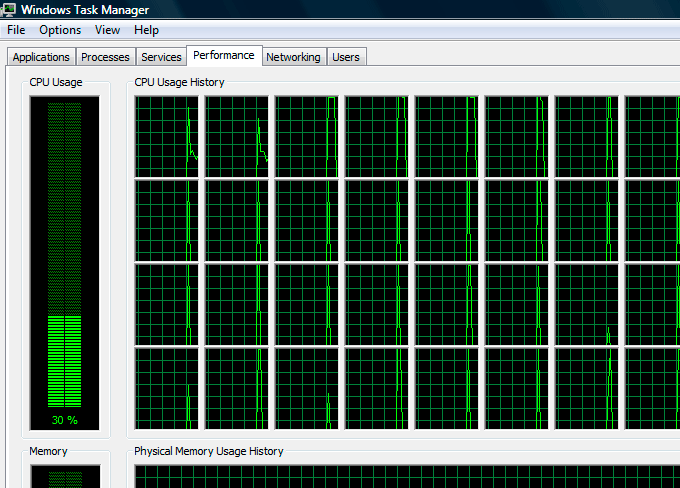
\includegraphics[scale=0.66]{exercises/taskmgr_64cpu_crop.png}
\caption{\IFRU{Обманутый}{Fooled} Windows Task Manager}
\end{figure}

\subsection{\Exercise 2.12}
% ROT13

\IFRU{Это довольно известный алгоритм}{This is a well-known algorithm}.
\IFRU{Как он называется}{How it's called}?

\subsubsection{MSVC 2012 x64 + \TT{/Ox}}

\lstinputlisting{exercises/1_12_MSVC_x64.asm}

\subsubsection{Keil (ARM)}

\lstinputlisting{exercises/1_12_ARM.s}

\subsubsection{Keil (thumb)}

\lstinputlisting{exercises/1_12_thumb.s}

\subsection{\Exercise 2.13}
% LFSR

\IFRU{Это довольно известный криптоалгоритм прошлого}{This is a well-known cryptoalgorithm of the past}.
\IFRU{Как он называется}{How it's called}?

\subsubsection{MSVC 2012 + \TT{/Ox}}

\begin{lstlisting}
_in$ = 8						; size = 2
_f	PROC
	movzx	ecx, WORD PTR _in$[esp-4]
	lea	eax, DWORD PTR [ecx*4]
	xor	eax, ecx
	add	eax, eax
	xor	eax, ecx
	shl	eax, 2
	xor	eax, ecx
	and	eax, 32					; 00000020H
	shl	eax, 10					; 0000000aH
	shr	ecx, 1
	or	eax, ecx
	ret	0
_f	ENDP
\end{lstlisting}

\subsubsection{Keil (ARM)}

\begin{lstlisting}
f PROC
        EOR      r1,r0,r0,LSR #2
        EOR      r1,r1,r0,LSR #3
        EOR      r1,r1,r0,LSR #5
        AND      r1,r1,#1
        LSR      r0,r0,#1
        ORR      r0,r0,r1,LSL #15
        BX       lr
        ENDP
\end{lstlisting}

\subsubsection{Keil (thumb)}

\begin{lstlisting}
f PROC
        LSRS     r1,r0,#2
        EORS     r1,r1,r0
        LSRS     r2,r0,#3
        EORS     r1,r1,r2
        LSRS     r2,r0,#5
        EORS     r1,r1,r2
        LSLS     r1,r1,#31
        LSRS     r0,r0,#1
        LSRS     r1,r1,#16
        ORRS     r0,r0,r1
        BX       lr
        ENDP
\end{lstlisting}

\subsection{\Exercise 2.14}
% GCD

\IFRU{Еще один хорошо известный алгоритм. Ф-ция берет на вход 2 значения и возвращает одно.}
{Another well-known algorithm. The function takes two variables and returning one.}

\subsubsection{MSVC 2012}

\index{ARM!\Instructions!CLZ}
\lstinputlisting{exercises/2/GCD_MSVC_2012_Ox.asm}

\subsubsection{Keil (ARM mode)}

\index{ARM!\Instructions!CLZ}
\lstinputlisting{exercises/2/GCD_Keil_ARM_O3.s}

\subsubsection{GCC 4.6.3 for Raspberry Pi (ARM mode)}

\index{x86!\Instructions!BSF}
\lstinputlisting{exercises/2/GCD_ARM_pi_GCC_4.6.3_O3.s}

\subsection{\Exercise 2.15}
% Monte Carlo

\IFRU{И снова известный алгоритм. Что он делает?}{Well-known algorithm again. What it does?}

\IFRU{Обратите внимание, что код для x86 использует FPU, а для x64 --- SIMD-инструкции. Это нормально}
{Take also notice that the code for x86 uses FPU, but SIMD-instructions are used instead in x64 code.
That's OK}: \ref{floating_SIMD}.

\subsubsection{MSVC 2012 x64 /Ox}

\lstinputlisting{exercises/2/monte_MSVC_2012_Ox_x64.asm}

\subsubsection{GCC 4.4.6 -O3 x64}

\lstinputlisting{exercises/2/monte_GCC_4.4.6_O3_x64.s}

\subsubsection{GCC 4.8.1 -O3 x86}

\lstinputlisting{exercises/2/monte_GCC_4.8.1_O3_x86.s}

\subsubsection{Keil (ARM mode): \IFRU{для процессора Cortex-R4F}{Cortex-R4F CPU as target}}

\lstinputlisting{exercises/2/monte_Keil_ARM_Cortex.s}

